\documentclass[10pt,aspectratio=169]{beamer}
%\setbeameroption{show only notes}

\usepackage{amsmath}

\usepackage{mypresento/config/presento}
\usepackage{tikz}
\usetikzlibrary{shadings,shadows,calc,backgrounds,positioning}
\usepackage{tcolorbox}
\usepackage{adjustbox}
\usepackage{bytefield}
\newcommand{\colorbitbox}[3]{%
    \rlap{\bitbox{#2}{\color{#1}\rule{\width}{\height}}}%
    \bitbox{#2}{#3}}
\tcbuselibrary{skins,breakable}

\usepackage{caption}

%\usepackage{transparent}
%\setbeameroption{show notes}

\usepackage[backend=bibtex,style=phys]{biblatex}
\bibliography{bib/myrefs}

\definecolor{darkblue}{HTML}{000099}
\usepackage{listings}
\lstset{
    frameround=fttt,
    language=C,
    numbers=left,
    %stepnumber=5,               % Abstand zwischen den Zeilennummern       
    %numberfirstline=false
    breaklines=true,
    keywordstyle=\color{black}\bfseries, 
    basicstyle=\ttfamily\footnotesize\color{darkblue},
    showstringspaces=false,
    numberstyle=\color{black},
	tabsize=2,
	columns=flexible,
	keepspaces=true
    }
\lstMakeShortInline[columns=fixed]|

% figures
\usepackage {pgf}                                 % includepgf for bitmaps
\usepackage{graphicx}

% Information
\title{Extending Compiler Support for the BrainScaleS Plasticity Processor}
\subtitle{Bachelor's Thesis Presentation}
\author{Arthur Heimbrecht}
\institute{}
\date{\today}

\begin{document}


% Title page
{
\usebackgroundtemplate{
    \tikz[overlay, remember picture]\node[opacity=0.2, inner sep=0, outer sep=0, ] at (current page.center) {\includegraphics[width=\paperwidth]{pictures/dls_die_photo.jpg}};
}
\begin{frame}[plain]
\maketitle
\note{ Welcome everybody to this talk about my Bachelor thesis. This might be a quite technical talk, please keep your questions until the end of the presentation.
Now the title of my thesis was Extending Compiler Support for the BrainScaleS Plasticity Processor.}
\end{frame}

}

\begin{frame}{Contents}
\begin{columns}[c]
    \begin{column}{.5\textwidth}
        \begin{minipage}[t][0.5\textheight]{0.75\textwidth}
            \tableofcontents[sectionstyle=show, subsectionstyle=show/show/shaded]
        \end{minipage}\hfill
    \end{column}

    \begin{column}{.5\textwidth}
        \centering
        \begin{figure}
            \includegraphics[width=\textwidth]{pictures/dls_die_photo.jpg}
            \caption{\label{fig:dls} Photograph of HICANN-DLS v1 chip, \citeauthor{PPU}}
        \end{figure}
    \end{column}
\end{columns}
\note{
    As the title hints there are two main components to this talk, which are the plasticity processing unit, or short PPU, and Compilers, specifically GCC.
	GCC is the compiler I used for this thesis.
    Afterwards I will explain the process of extending GCC, which is of course followed by a short presentation of the results as well as an outlook.

    But first I should explain, what the PPU is.
}
\end{frame}

% sections in the presentation
\section{PPU Architecture}
\begin{frame}{HICANN-DLS}
    \begin{columns}[c]
    \begin{column}{0.5\textwidth}
        \centering
		\vspace*{1em}
        \begin{figure}
                \begin{adjustbox}{center, max width={.50\columnwidth}}
                    
\noindent{\begin{minipage}{\textwidth}
   
\begin{tikzpicture}[style={circle,draw,fill=black,minimum size=15}, line width=.5mm]
       \foreach \x in {0,...,31}
           \foreach \y in {0,...,31} 
                  {\pgfmathtruncatemacro{\label}{\x - 5 *  \y +21}
                  \node [circle,draw,fill=black,minimum size=0.1, inner sep = 0pt]  (\x\y) at (0.3*\x,0.3*\y) {};}
   \end{tikzpicture}
\end{minipage}}

                \end{adjustbox}
			\vspace*{-1em}
            \caption{\label{fig:array} Schematic Representation of the Synapse Array on HICANN-DLS v2 and newer}
        \end{figure}

    \end{column}

    \begin{column}{0.5\textwidth}
        \centering
        \begin{figure}
            \includegraphics[width=\textwidth]{pictures/dls_marked.pdf}
            \caption{\label{fig:dls} Photograph of the HICANN-DLS v1 Chip, modified from \citeauthor{PPU}}
        \end{figure}
    \end{column}
    \note{\tiny
        I am assuming that everybody here likely has heard about the HICANN-DLS.
        In short it is a chip that emulates neural networks through neurons and synapses that are implemented directly on the chip.
        What is special about the DLS, is the addition of a PPU to the HICANN system.
        The PPU is capable of performing simple computation and allows for on-line plasticity directly on the chip itself.

        As you can see to the right I have marked the physical compartments on the HICANN-DLS.
        First we have the neurons.
        There are 32 neurons on the HICANN-DLS and each neuron is a circuit that receives some input signal which can cause the neurons to spike.
        These signals come from the so called synapse array.
        It connects 32 pre-synaptic inputs to all 32 neurons down here.
        This gives a total of 1024 synapses on each HICANN-DLS v2 and newer versions.
        
        Each synapse is realized through a circuit that takes the input signal and modifies it with a synpatic weight, that is saved in each synapse.
        Each synaptic weight is 6 bits wide, which is equivalent to numbers between 0 and 63.
        
        The pre-synaptic inputs are handled by an FPGA, that takes care of spike routing.
        
        But there is also a correlation analog digital converter, that measures correlation which can read out by the PPU as well. 

        The PPU is spread on this remaining large section of the HICANN-DLS chip.
		Most of this is based on an existing processor architecture, that is called PowerISA, but it was extended with a custom vector extension for the PPU.

		Now I want to talk a little about processors in general and apply this to the PPU.
}
    \end{columns}
\end{frame}

\begin{frame}{Processors}
    \begin{columns}[c]
    \begin{column}{0.5\textwidth}
		\begin{itemize}[<1->]
			\setlength\itemsep{1em}
            \item ``common'' von-Neumann architecture
			\item machine instructions in memory
			\item data in memory
            \item<2-> latency(register) $\approx$ 1 cycle
			\item<2-> latency(memory) $\approx$ 100-1000 cycles
		\end{itemize}
    \end{column}

    \begin{column}{0.5\textwidth}
        \centering
        \vspace*{3em}
        \begin{figure}
                \begin{adjustbox}{center, max width={.7\columnwidth}}
                    \chapter{Processor basics}
\label{chapter:processor}

Next to all processors used these days are built upon the so called von-Neumann architecture \todo{add reference}.
\todo{cite freidmann dissertation}Though the main goal of this group is to provide an alternative analogue architecture that is inspired by nature, there are advantages to the classic model of processors which are needed at some point.
The main advantage of digital systems over analogue systems such as the human brain, is the ability to do calculations at much higher speeds.
For this reason ``normal" processors are responsible for handling experiment data as well as setting up different parts of the experiment.
One such task is applying learning rules to the synapses during or in between experiments which can either be done by hand or with the help of the aforementioned PPU.
The second option is especially valuable when updating synaptic weights during an experiment as the PPU does this much faster than a system which interacts from the outside.
This is important for achieving experimental speeds that are $10^{4}$ times faster than their biological counterparts.

Therefore the PPU is one of many von-Neumann processors in this world and follows the same basic concepts.
It is important to understand these concepts as they build the foundation to this report!



ALU
FPU
memory
memory controller
clockcycle
pipeline


                \end{adjustbox}
            \caption{\label{fig:processor} Schematic of General Purpose Processor with von-Neumann Architecture}
        \end{figure}
    \end{column}
    \end{columns}
\note{	
		As you may know, next to all computing nowadays is done by processors which are often described as CPUs.
		The processors are normally built according to the von-Neumann architecture, which combines programs and data in the same memory.
		The processor fetches so called machine instructions from the memory and analyzes them to decide what to do.
		This is what we call the computer running a program.
		All computation on processors like the PPU is not done in memory but in registers.
		These registers can only hold small amounts of data, usually one variable, but offer a very low access time compared to memory.
		Still, data can be exchanged between registers and memory to save results or load values.
		Using memory usually takes a significant amount of time longer than access to registers and thus programs should try to use registers as much as possible.
}

\end{frame}

\begin{frame}{Plasticity Processing Unit}
    \begin{columns}[c]
    \begin{column}{0.5\textwidth}
        \begin{itemize}
			\setlength\itemsep{1em}
			\item based on PowerISA
            \item extension with vector registers \\ \hspace{10mm}
				$\rightarrow$ parallelization of operations\\ \hspace{10mm}
				$\rightarrow$ better performance
            \item weight updates
			\item access to synaptic array
        \end{itemize}
    \end{column}

    \begin{column}{0.5\textwidth}
        \centering
        \begin{figure}
            \includegraphics[width=.8\textwidth]{pictures/nux.pdf}
            \caption{\label{fig:nux} Structure of nux Architecture}
        \end{figure}
    \end{column}
    \end{columns}
\note{	
		In addition to this, the PPU offers another kind of register which are vector registers.
		These are part of a special vector extension which was added to the PPU base architecture.
		Using vector registers is favorable for operations that use have to be applied to multiple values and can be done in parallel.
		
		And this is the strength of the PPU as is allows to compute weight updates for up to 16 synapses at the same time in a single register, as normally only a single value could be handled by a register.
		This increases performance significantly, especially since the are many synapse weight on a single chip. 
		
		For this reason the PPU is also connected to the synaptic array and is able to read out and write synaptic weights to the vector registers.

		But this induces a problem because the vector extension of the PPU uses special machine  instructions that are unique to the PPU's architecture.
}
\end{frame}



\section{Compiler Structure}
\begin{frame}[fragile]{Compiler Structure}
    \begin{columns}[c]
    \begin{column}{0.5\textwidth}
        \begin{itemize}
			\setlength\itemsep{1em}
            \item code $\xrightarrow{\text{compile}}$ executable
			\item different compiling stages (e.g. Preprocessor)
			\item front-end $\rightarrow$ programming language
			\item middle-end $\rightarrow$ optimization
			\item back-End $\rightarrow$ processor architecture
        \end{itemize}
    \end{column}

    \begin{column}{0.5\textwidth}
        \centering
        \begin{figure}
            \begin{adjustbox}{center, max width={.6\columnwidth}}
				    \tcbset
    {my box/.style={enhanced,colframe=blue!70!black,colback=white!50!blue,colupper=red!50!black,
        fonttitle=\bfseries,nobeforeafter,center title, noparskip, size=small},
    every box on layer 1/.style={every box},
    every box on layer 2/.style={reset,my box}}
\begin{tcolorbox}[enhanced jigsaw, width=\textwidth, opacityframe=0.0, opacityback=0.0]
\begin{tcolorbox}[enhanced, height=.5cm, width=\linewidth, remember as=pp, opacityframe=0.0, opacityback=0.0]\end{tcolorbox}
\begin{tcolorbox}[enhanced, height=.7cm, width=\linewidth, watermark text=Preprocessor, remember as=pp]\end{tcolorbox}
\begin{tcolorbox}[tcbox raise base, width=\linewidth, enhanced jigsaw, remember as=cmp]
    \begin{tcolorbox}[enhanced, breakable, noparskip,opacityframe=0.3, opacityback=0.3, height=1.4cm, width=\linewidth, watermark text=Front-End, remember as=fe]
    \end{tcolorbox}
    \begin{tcolorbox}[enhanced, breakable, noparskip,opacityframe=0.3, opacityback=0.3, height=0.7cm, width=\linewidth, watermark text=Middle-End, remember as=me]
    \end{tcolorbox}
    \begin{tcolorbox}[enhanced, breakable, noparskip,opacityframe=0.3, opacityback=0.3, height=1.1cm, width=\linewidth, watermark text=Back-End, remember as=be]
    \end{tcolorbox}
\end{tcolorbox}

\end{tcolorbox}

\begin{tikzpicture}[overlay,remember picture,line width=1mm]
    \draw[->, shorten >=-1.5mm] ($(pp.north)+(0,1.5)$) -- node [left] {program code} (pp.north);
    \draw[->, shorten >=-1.5mm] (pp.south) -- (fe.north);
    \draw[->, shorten >=-1.5mm] (fe.south) -- (me.north);
    \draw[->, shorten >=-1.5mm] (me.south) -- (be.north);
    \draw[->] (be.south) -- node [left] {machine files} ++(0,-1.5);
\end{tikzpicture}

            \end{adjustbox}
            \caption{\label{fig:compiler} Structure of Compiling Process and Compiler}
        \end{figure}
    \end{column}
    \end{columns}
\note{	\scriptsize
		This is of special significance when using a compiler.
		But why?
		As most people usually do not code in machine language but use a high-level language like C, compilers translate this language into specific machine instruction.
		This is necessary so the computer can run the program.
		
		Compiler usually consist of several compiling stages in a pipeline that follow different purposes, like the preprocessor.
		It takes care of substituting macros and including header files in program code.
		The actual compiler will then take the preprocessed code and create machine files from this.

		As you can see, there are different phases in the compiler itself which are responsible for different tasks.
		The front-end reads the program so the compiler understands it.
		Having different front-ends allows to use different languages for the same compiler.

		The middle-end is specific to different compilers and handles general optimization.
		
		The back-end is mainly responsible for creating the actual machine code from input by the front-end and middle-end.
		It also optimizes the code it generated.
		All this only applies to a specific processor architecture which the back-end is build for.
		Exchanging back-ends would allow to run the same code on various machines with different processor architectures.
		One architecture, that most of you might know is the ARM architecture that is at the heart of every smartphone and also SpiNNaker.
		Another is x86 which is at the core of basically every home computer.

		The PPU though, is based on yet another architecture, as I already mentioned.}
\end{frame}

\begin{frame}[fragile]{GCC and the PPU}
    \begin{columns}[c]
    \begin{column}{0.5\textwidth}
        \begin{itemize}
			\setlength\itemsep{1em}
            \item no ``official'' support for PPU
			\item currently using macros
			\item<3-> existing AltiVec extension
			\item<4-> intrinsics $\rightarrow$ \textbf{use this}
        \end{itemize}
    \end{column}

    \begin{column}{0.5\textwidth}
        \centering
		\begin{visibleenv}<1->
				\begin{lstlisting}[title=Example for macro usage]
#define VR_TMP     0
#define VR_A       1
...
fxv_addbm(VR_A, VR_A, VR_TMP);
				\end{lstlisting}
	\end{visibleenv}

		\begin{visibleenv}<2->
				\begin{lstlisting}[title=Preprocessed example]
...
fxv_addbm(1, 1, 0);
				\end{lstlisting}
	\end{visibleenv}

		\begin{visibleenv}<3->
				\begin{lstlisting}[title=Example for AltiVec code]
vector char a, tmp;
...
a = vec_add(a, tmp);
				\end{lstlisting}
	\end{visibleenv}
    \end{column}
    \end{columns}
\note{\scriptsize	Of course there exist different compilers and one which is used by this group is the GNU Compiler Collection, or just GCC.
		GCC is a compiler that is wide-spread especially at academic institutions.
		It is capable of compiling a large variety of languages for most processor architectures that exist.
		Unfortunately this does not include the PPU's architecture.
		Although the basic architecture of the PPU IS supported, there is no official GCC support of the vector extension.

		This means that users can code in C for example but every time they need to use the vector extension, it is necessary to handle low level code, which is quite tricky.
		And most users wouldn't know how to do this.
		There have been efforts to make this easier, but still it mostly looks like this when programming for the PPU.
		<bild zeigen>
		It uses macros for low level programming where registers must be allocated by hand.
		And if you still remember what registers are from 5 minutes ago, it might be clear that this is tedious work.
		And if you don't already understood the problem of coding like this.

		But there ARE easier ways to program for vector extensions.
		One such extension is the AltiVec extension.
		Some Mac users might know this as is was an extension to the PowerISA used by Apple before they switched to Intel.
		Back in the day it was a huge selling point to offer easy vector programming like this to users.
		<zweites bild>
		It uses so called intrinsics for vector processing, which are basically functions with certain input variables and a return value.

		And if we compare these two examples, I think it becomes clear that the second one is way easier and what you would like vector programming to look like.
		Users do not have to learn about registers as they can still use variables.
		The structure of complex programs is still clear to the user and overall we can stick to one programming language.

		This is important for new users that want to code for the PPU as well as experienced users that have to rearrange and manage  registers for complex programs.
}
\end{frame}


\section{Extending GCC for the PPU}
\begin{frame}[fragile]{Main Work of this Thesis}
    \begin{columns}[c]
    \begin{column}{0.5\textwidth}
		\begin{itemize}[<+->]
			\setlength\itemsep{1em}
            \item Add GCC support for PPU
			\item GCC back-ends not documented
			\item AltiVec inspiration for\\\hspace{2em}
				Internal functions\\\hspace{2em}
				Internal macros
			\item Other Components:\\\hspace{2em}
				Vector Registers\\\hspace{2em}
				Vector variables\\\hspace{2em}
				New intrinsics\\\hspace{2em}
					...
        \end{itemize}
    \end{column}

    \begin{column}{0.5\textwidth}
				\begin{lstlisting}[title=Previous PPU code]
#define VR_TMP     0
#define VR_A       1
...
fxv_addbm(VR_A, VR_A, VR_TMP);
				\end{lstlisting}
				\hspace*{3em}\tikz{\draw[->, line width=1mm] (0,0) -- node [right] {This thesis} ++(0,-1.0);}
				\begin{lstlisting}[title=New PPU code]
vector char a, tmp;
...
a = fxv_add(a, tmp);
				\end{lstlisting}
			
    \end{column}
    \end{columns}
\note{	So this was the motivation for my Bachelor's thesis.
		I want to simplify programming on the PPU for new users as well as experienced users, which should help making use of the PPU's capabilities.

		To do so, I extended the GCC compiler we already used for the PPU, in order to make PPU programming more similar to AltiVec programming.

		And as simple as it sounds at first it was quite a challenge, since there was no documentation of the PowerISA back-end except comments and general information on how to create some back-end in GCC.
		This makes sense, as usually processors are usually not customized like that.
		And if they are customized, that is done by corporations like Intel, with special people managing compiler support.

		Luckily there is already this AltiVec extension, which I mentioned earlier, and it provided a good guideline for me to find relevant sections in the back-end's code.

		Ultimately I had to go through roughly 50.000 lines of code that make up the back-end and it needed about 3.000 additional lines to add support for the PPU.
		This included things like:
			creating a new vector register type
			adding a vector variables
			building intrinsics for each vector instruction on the PPU
			and so on
		
		Most work actually went into adding supportive functions and macros which were needed to make the back-end work at all.

		But instead of going further into detail I want to show you the results of this and also give an outlook, of what might be possible in the future.
}
\end{frame}

\section{Results}
\begin{frame}[fragile]{New Features}
    \begin{columns}[c]
    \begin{column}{0.5\textwidth}
		\begin{itemize}[<+->]
			\setlength\itemsep{1em}
			\item |-mcpu=nux| target flag \& |s2pp.h| header
			\item |vector| attribute for variables
			\item simple vector construction
			\item PPU vector intrinsics
			\item inline assembly support
			\item optimization
        \end{itemize}
    \end{column}

    \begin{column}{0.5\textwidth}
        \centering
		\begin{onlyenv}<1>
				\begin{lstlisting}[title=Compiling Directive]
powerpc-linux-eabi-gcc -mcpu=nux
				\end{lstlisting}
				
				\begin{lstlisting}[title=Example File]
				#include<s2pp.h>
				
				start(){
				  return;
				}
				\end{lstlisting}
				\vspace{5em}
	\end{onlyenv}
		\begin{onlyenv}<2>
				\begin{lstlisting}[title=Compiling Directive]
powerpc-linux-eabi-gcc -mcpu=nux
				\end{lstlisting}
				\begin{lstlisting}[title=Example File]
				#include<s2pp.h>

				start(){
				  vector char vec;
				  return;
				}
				\end{lstlisting}
				\vspace{4em}
	\end{onlyenv}
		\begin{onlyenv}<3>
				\begin{lstlisting}[title=Compiling Directive]
powerpc-linux-eabi-gcc -mcpu=nux
				\end{lstlisting}
				\begin{lstlisting}[title=Example File]
				#include<s2pp.h>

				start(){
				  vector char vec = 
				      {1,1,1,1,1,1,1,1,1,1,1,1,1,1,1,1};
				  return;
				}
				\end{lstlisting}
				\vspace{3em}
	\end{onlyenv}
		\begin{onlyenv}<4>
				\begin{lstlisting}[title=Compiling Directive]
powerpc-linux-eabi-gcc -mcpu=nux
				\end{lstlisting}
				\begin{lstlisting}[title=Example File]
				#include<s2pp.h>

				start(){
				  vector char vec = 
				      {1,1,1,1,1,1,1,1,1,1,1,1,1,1,1,1};
				  vec = fxv_add(vec, vec);
				  return;
				}
				\end{lstlisting}
				\vspace{2em}
	\end{onlyenv}
		\begin{onlyenv}<5>
				\begin{lstlisting}[title=Compiling Directive]
powerpc-linux-eabi-gcc -mcpu=nux
				\end{lstlisting}
				\begin{lstlisting}[title=Example File]
				#include<s2pp.h>

				start(){
				  vector char vec = 
				      {1,1,1,1,1,1,1,1,1,1,1,1,1,1,1,1};
				  vec = fxv_add(vec, vec);
				  asm ("fxvaddbm %0, %0, %0"
				      :"+kv" (vec)::);
				  return;
				}
				\end{lstlisting}
	\end{onlyenv}
		\begin{onlyenv}<6>
				\begin{lstlisting}[title=Compiling Directive]
powerpc-linux-eabi-gcc -mcpu=nux -O1
				\end{lstlisting}
				\begin{lstlisting}[title=Example File]
				#include<s2pp.h>
				
				start(){
				  vector char vec = 
				      {1,1,1,1,1,1,1,1,1,1,1,1,1,1,1,1};
				  vec = fxv_add(vec, vec);
				  asm ("fxvaddbm %0, %0, %0"
				      :"+kv" (vec)::);
				  return;
				}
				\end{lstlisting}
	\end{onlyenv}
    \end{column}
    \end{columns}
\note{	Let's start on the prerequisites on generating code for the PPU with the extended Compiler.
		It simply takes one target flag -mcpu=nux and a header file s2pp.h, to create code, which is compatible with the PPU.
		This was several flags before which are all combined in this directive.
		<bild>
		Also there is a vector type which can be used to represent vectors as variables and it works exactly like other existing vector attributes especially AltiVec.
		The vector's type gives the size of an element and the compiler creates a whole vector with all elements being the same size.
		<extend picture>
		It now very easy to initialize these vectors as well, because it does not need arrays or similar things to set specific values.
		You can simple list all elements like this and the compiler will construct the according vector.
		<bild>
		Most importantly, users can now use intrinsics for simple vector instructions and use the vector variables instead of arbitrary macros or register numbers.
		This definitely makes a difference as is complies for existing standards in coding.
		<extend picture>
		Furthermore, there is inline assembly support which allows for low level coding whenever it is needed.
		Although this was also possible before, but again there is no need for handling registers yourself.
		You can simply add instructions and the compiler will assign register and handle variable in memory.
		<extend picture>
		And all of this also supports simple optimization, that allows for more efficient programs on the PPU, without particular low-level knowledge by the user.
		As of now only the lowest form of optimization is safely supported but as you can see on the next slide, this already reduces program size significantly.
		And this increases performance as well.
}
\end{frame}

\begin{frame}[fragile]{Advantages}
    \begin{columns}[c]
    \begin{column}{0.4\textwidth}
		\begin{itemize}[<2->]
			\setlength\itemsep{1em}
            \item easier PPU programs for users
			\item efficient programs
			\item workarounds in compiler
			\item C-library support for PPU\\\hspace{2em} $\rightarrow$ soft-float
        \end{itemize}
    \end{column}

    \begin{column}{0.6\textwidth}
        \centering
		\scriptsize Comparison of unoptimized code (left) and |-O1| optimized code (right)
            \begin{adjustbox}{center, max width={1\columnwidth}}
			\begin{lstlisting}[basicstyle=\ttfamily\tiny\color{darkblue}]
start:
	stwu %r1,-64(%r1)
	stw %r31,60(%r1)
	mr %r31,%r1
	li %r9,1
	fxvsplatb %f12,%r9
	li %r9,16
	fxvstax %f12,%r31,%r9
	li %r9,16
	fxvlax %f12,%r31,%r9
	li %r9,16
	fxvlax %f11,%r31,%r9
	fxvaddbfs %f12,%f12,%f11
	li %r9,16
	fxvstax %f12,%r31,%r9
#APP
 # 277 "nux/main.c" 1
	fxvaddbm %f12, %f12, %f12
 # 0 "" 2
#NO_APP
	li %r9,16
	fxvstax %f12,%r31,%r9
	nop
	addi %r11,%r31,64
	lwz %r31,-4(%r11)
	mr %r1,%r11
	blr
			\end{lstlisting}
			\hspace*{2em}
			\begin{lstlisting}[basicstyle=\ttfamily\tiny\color{darkblue}]
start:
	stwu %r1,-48(%r1)
	li %r9,1
	fxvsplatb %f12,%r9
	li %r9,16
	fxvstax %f12,%r1,%r9
	fxvlax %f12,%r1,%r9
	fxvlax %f11,%r1,%r9
	fxvaddbfs %f12,%f12,%f11
	fxvstax %f12,%r1,%r9
#APP
 # 277 "nux/main.c" 1
	fxvaddbm %f12, %f12, %f12
 # 0 "" 2
#NO_APP
	fxvstax %f12,%r1,%r9
	addi %r1,%r1,48
	blr
			\end{lstlisting}
            \end{adjustbox}
    \end{column}
    \end{columns}
\note{
	So just to summarize the advantages I mentioned:
		We have easier code that allow new user an easier introduction and experienced users better structured programs
		These programs are also efficient without assistance of the user.
		Although I have to say that a good low level programmer will always produce better code than the compiler, and with the current state PPU software looses a little performance.
		But with more optimization stages this gap will shrink.

		Also during my thesis David Stoeckel and I found a PPU bug which can be worked around inside the compiler and does not need any changes in software.

		Also the compiler support might allow some C-libraries to work on the PPU as well and give us features like soft-float numbers.

		All in all this should help a great deal in creating new and exciting experiments which involve the PPU.
		
}
\end{frame}

\begin{frame}[fragile]{Outlook}
    \begin{columns}[c]
    \begin{column}{0.5\textwidth}
		\begin{itemize}[<1->]
			\setlength\itemsep{1em}
			\item further testing for compiler bugs
			\item already existing applications
			\item extending PPU test coverage
			\item debugging support?
			\item<2-> \textbf{new tools for PPU experiments!}
			\item<3-> \textbf{more experiments!}
        \end{itemize}
    \end{column}

    \begin{column}{0.5\textwidth}
        \centering
				\begin{lstlisting}[title=Compiling Directive]
powerpc-linux-eabi-gcc -mcpu=nux -O1
				\end{lstlisting}
				\begin{lstlisting}[title=Example File]
				#include<s2pp.h>
				
				start(){
				  vector char vec = 
				      {1,1,1,1,1,1,1,1,1,1,1,1,1,1,1,1};
				  vec = fxv_add(vec, vec);
				  asm ("fxvaddbm %0, %0, %0"
				      :"+kv" (vec)::);
				  return;
				}
				\end{lstlisting}
    \end{column}
    \end{columns}
\note{	\scriptsize
		So what will the future bring for the compiler?

		I have to mention that it still is kind of in a beta phase and that there are bugs that can occur.
		But this is somewhat normal when creating new software and even compilers.
		Ultimately the more people will use this compiler, the more bugs can be fixed over time and this will become an even more handy tool, when programming for the PPU.
		It is there a good idea to create tests for the compiler that test stability of programs and at various optimization stages.
		
		Nonetheless there already exist programs and tests that make use of the compiler extension.

		David Stoeckel for example used it to test criticality for his presentation a few weeks ago.
		He also used a low level support library that allows for simple tests and PPU output on the console.
		I really recommend using it when conducting your first experiments with the PPU.

		There are also first highlevel PPU tests that use the compiler and these helped in finding the PPU bug I addressed earlier.
		\\
		\\
		And there is more of what might be possible in the future with compiler support for the PPU.

		For once it will be easier to create more high-level tests for the PPU and extending the current test coverage is something I would like to do in the future to rule out any other PPU bugs.
		Also it might be possible to realize debugging support for the PPU, but this is something that is not yet on the agenda.

		All in all I want to encourage as many of you as possible to use the new compiler as a tool when conductin experiments with the PPU.
		The compiler offers easier programming for the PPU than ever before and it will become better over time as more users develop with it.
		And it might pave the way for more experiments in the near future that include the PPU which IS a key feature of the HICANN-DLS.
		As we ultimately want to use all capabilities of our system.

		So this was my thesis talk and I would be happy if I was able to interest some of you in experiments involving the PPU which will make use of the new compiler.
}
\end{frame}

\appendix

\setbeamerfont{caption}{size=\tiny}


\section{Appendix}
\nocite{PPU}
\nocite{microprocessor}
\nocite{UBHD-67548259}
\nocite{UBHD-66483012}
\nocite{nuxmanual}
\nocite{GCCint}

\begin{frame}[fragile]{References}
	\vspace*{3em}
	{\scriptsize
	\printbibliography}
\end{frame}

\scriptsize

\begin{frame}[fragile]{Additional Figures}
	\vspace*{2em}
	\begin{columns}[t]
		\begin{column}{.5\textwidth}
\begin{figure}
    \centering
    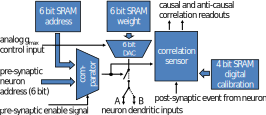
\includegraphics[width=\textwidth]{pictures/syncircuit.pdf}
    \caption{\label{fig:circuit} Block Diagram of the Synapse Circuit (modified from~\citeauthor{PPU}).}
\end{figure}
	\vspace*{-1em}
\begin{figure}
    \centering
    \begin{bytefield}[endianness=big, bitwidth=0.027777\linewidth, bitheight=2em]{32}
        \bitheader{0,7,15,23,31}\\
        \bitboxes{8}{{mnemonic}{operand}{operand}{operand}}\\
        \bitboxes{8}{{\tt{addi}}{{\tt r1} \\ \tiny register address}{{\tt r2} \\ \tiny register address}{{\tt 5} \\ \tiny immediate operand}}
    \end{bytefield}
    \caption{\label{fig:mnemonic} Representation of Assembly Instruction {\tt addi} as a Machine Instruction in Memory. The immediate value {\tt 5} is added to register {\tt r2} and the result written in {\tt r1}.}
\end{figure}
		\end{column}
		\begin{column}{.5\textwidth}

\begin{figure}
    \centering
    \includegraphics[width=\textwidth]{pictures/s2pp.pdf}
    \caption{\label{fig:s2pp} Detailed Structure of the s2pp Vector Extension (taken from~\citeauthor{PPU})}
\end{figure}

\begin{figure}[htpb]
    \centering
		\scriptsize
        \begin{bytefield}[bitwidth=0.11111111\textwidth, bitheight=2em]{8}
            \bitheader[endianness=big]{0-7}\\
            \bitbox{1}{\color{lightgray}\rule{\width}{\height}} & \bitbox{1}{\color{lightgray}\rule{\width}{\height}} & \bitbox{1}{$2^{5}$} & \bitbox{1}{$2^{4}$} & \bitbox{1}{$2^{3}$} & \bitbox{1}{$2^{2}$} & \bitbox{1}{$2^{1}$} & \bitbox{1}{$2^{0}$}\\
        \end{bytefield}
    \caption{\label{fig:fractional} Comparison of the Representation of Weights in Synapses and the Fractional Representation of Vector Components for Fixed-Point Saturational Arithmetic}
\end{figure}

		\end{column}
	\end{columns}

\end{frame}
\begin{frame}[fragile]{Additional Figures}

\begin{figure}
	\vspace*{3em}
    \centering
	\begin{bytefield}[endianness=little, bitwidth=\widthof{\tiny bit}/2, bitheight=2em]{128}
        \bitheader{0,7,15,31,63,127}\\
    \bitboxes{8}{{QI}{\tiny Quarter \\ Integer}{}{}{}{}{}{}{}{}{}{}{}{}{}{}}\\
    \bitboxes{16}{{HI}{\tiny Half \\ Integer}{}{}{}{}{}{}}\\
	\bitboxes{32}{{SI}{\tiny Single \\ Integer}{}{}}\\
    \bitboxes{32}{{SF}{\tiny Single \\ Float}{}{}}\\
    \end{bytefield}
	\vspace*{-1.5em}
    \caption{\label{fig:vectorlength} Vector structures are 128 bits wide and split into common word sizes.}
\end{figure}

\begin{figure}
	\begin{bytefield}[endianness=little, bitheight=2em, bitwidth=\widthof{\tiny bit}]{32}
        \bitheader{0,1,7,15,31}\\
        \colorbitbox{lightgray}{1}{\tiny bit} && \bitbox{31}{}\\
        \colorbitbox{lightgray}{8}{byte} && \bitbox{24}{}\\
        \colorbitbox{lightgray}{16}{halfword} && \bitbox{16}{}\\
        \colorbitbox{lightgray}{32}{word}\\
    \end{bytefield}
	\vspace*{-1.5em}
    \caption{\label{fig:bitlength} Illustration of Word Sizes for 32-bit Words}
\end{figure}

\end{frame}

\end{document}
